\documentclass[10pt, xcolor=pdflatex, dvipsnames, table]{beamer}
%------------------  xcolor,         jmena barev, colortbl/rowcolors

%\usepackage{czech}    % pokud chceme ceske labely
\usepackage{graphicx}  % obrazky
\usepackage{newcent}   % Century Gothic FONT

\usetheme[tocnumbers]{FIT} 
\usepackage{ucs}
\usepackage[utf8x]{inputenc}
\usepackage[czech]{babel}
\usepackage{palatino}
\usepackage{graphicx}
\usepackage{textcomp}
\usepackage{algorithm}
\usepackage{algorithmicx}
\usepackage{algpseudocode}
\usepackage{wrapfig}

\title{Design and Performance Analysis of Parallel
Processing of SRTP Packets}
\author{Jan Wozniak}
\institute[FIT VUT]{Vysoké učení technické v~Brně\\
Fakulta informační technologií}
\date{\today}

\begin{document}

\begin{frame}[plain]
\titlepage
\end{frame}


\begin{frame}
\frametitle{Parallel Processing of SRTP}

\begin{wrapfigure}[3]{r}[0em]{0em}

\includegraphics[width=3cm]{img/OpenCL_Logo.png}
\end{wrapfigure}

\textbf{Open Computing Language} 
\begin{itemize}
  \item standard for parallel computations
  \item wide support of HW and SW
  \item active contributions 
  \item many important vendors (including Apple, AMD, intel)
\end{itemize} 

\vspace{1.5em}

\textbf{SRTP parsing}
\begin{itemize}
\item usual size 2 to 10 AES blocks
\item careful allocation of resources vs. massive parallelization -- 
persistent thread paradigm
\item minimize average delay caused by packet processing on gateway
\end{itemize}
\end{frame}






\begin{frame}
\frametitle{Application Design}
\begin{figure}[H]
\centering
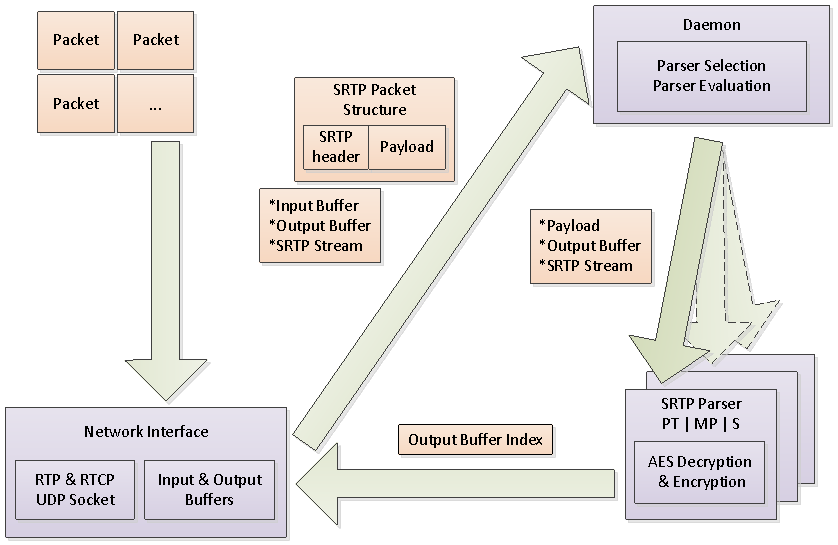
\includegraphics[width=10cm,keepaspectratio]{img/eeit.pdf}
\end{figure}
\end{frame}





\begin{frame}
\frametitle{Results}
\footnotesize{Following graphs visualize distribution of packet delays in \textit{ms} over
\textit{number of concurrent calls} using G.711 with sampling period 20ms during test.}

\begin{figure}[H]
\centering
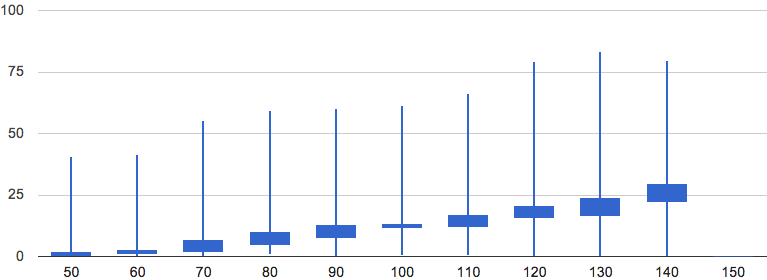
\includegraphics[width=8cm,keepaspectratio]{img/cpu.png}

\footnotesize{\textbf{Figure:} Serial implementation.}
\end{figure}

\vspace{-1em}

\begin{figure}[H]
\centering
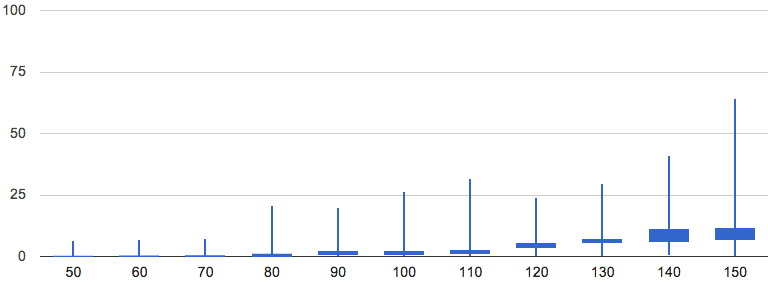
\includegraphics[width=8cm,keepaspectratio]{img/gpu.png}

\footnotesize{\textbf{Figure:} Parallel implementation.}
\end{figure}
\end{frame}





\begin{frame}
\frametitle{Conclusion}
\textbf{Compiled and tested using:}
\begin{itemize}
\item processor -- intel core i5 2500k
\item operating system -- OpenSUSE 12.2
\item used languages, frameworks and libraries 
  \begin{itemize}
  \item C/C++ std=c++11 (compiled with gcc 4.7)
  \item OpenCL 1.2
  \item Boost 1.53.0
  \end{itemize}
\end{itemize}

\vspace{1em}

\textbf{Results:}
\begin{itemize}
\item Average packet delay caused by SRTP encryption
  \begin{itemize}
    \item dropped to one third during 140 concurrent calls 
    \item at least to half during smaller amount of concurrent calls
  \end{itemize}
\end{itemize}
\end{frame}


\frame[plain]{\bluepage{}}
\end{document}
